% W3PHIAI-27 (AAAI-27 workshop on Health Intelligence) short paper: at most 4 pages including references, so that
% the full version stays eligible for CHIL 2027 (which accepts extensions of published papers of at most 4 pages).
% Single-blind. Template: AAAI-27 Author Kit (aaai2027.sty, aaai2027.bst), unmodified.
\documentclass[letterpaper]{article} % DO NOT CHANGE THIS
\usepackage{aaai2027}  % DO NOT CHANGE THIS
\usepackage[hyphens]{url}  % DO NOT CHANGE THIS
\usepackage{graphicx} % DO NOT CHANGE THIS
\urlstyle{rm} % DO NOT CHANGE THIS
\def\UrlFont{\rm}  % DO NOT CHANGE THIS
\usepackage{natbib}  % DO NOT CHANGE THIS AND DO NOT ADD ANY OPTIONS TO IT
\usepackage{caption} % DO NOT CHANGE THIS AND DO NOT ADD ANY OPTIONS TO IT
\frenchspacing  % DO NOT CHANGE THIS
\setlength{\pdfpagewidth}{8.5in} % DO NOT CHANGE THIS
\setlength{\pdfpageheight}{11in} % DO NOT CHANGE THIS
\usepackage{booktabs}
\newcommand{\passk}[1]{\mathrm{pass@}#1}
\pdfinfo{
/TemplateVersion (2027.2)
}
\setcounter{secnumdepth}{0}

\title{Stated or Sampled? Pass@$k$, Voting and Agreement Misjudge the\\Differential Diagnoses of Post-Trained LLMs Answering Directly}
\author{
    Author Name\textsuperscript{\rm 1}
}
\affiliations{
    \textsuperscript{\rm 1}Affiliation\\
    email@example.com
}

\begin{document}
\maketitle

\begin{abstract}
A language model's differential diagnosis can be read from the list of conditions it states in one answer, or from the spread of its answers over repeated samples. Pass@$k$, majority voting and agreement-based uncertainty all use the second. We compare both readouts in base and post-trained versions of open 4--72B models on 980 synthetic DDXPlus patients and 897 published case reports. Post-training collapses the samples: post-trained models give 1.3--2.4 distinct answers in 32 samples instead of 3.0--4.9, and lose 12--30 points of pass@32 (at each model's best prompt; 6--18 after correcting for chance). The single stated list does not collapse. For 7--20\% of patients, a post-trained model's first list names the true diagnosis while none of its 32 samples does, and on the case reports one list covers the alternatives the authors considered as well as before, while 32 samples cover 8--14 points fewer in four of five pairs. Tools built on samples suffer: voting adds at most 2 points, and every other sample repeats 19--61\% of post-trained models' wrong answers, so agreement cannot flag them. Evaluations of post-trained models should say which readout they use, and systems that need several candidates should read them from the stated list.
\end{abstract}

\section{Introduction}
Clinicians reason over a differential diagnosis, the ranked set of conditions that could explain a presentation; it decides which tests are ordered and which dangerous possibilities are ruled out. A language model's differential can be read in two ways: from the list it \emph{states} in one answer, or from the distribution of its answers over repeated \emph{samples}. Clinical evaluations have scored the lists models state~\citep{mcduff2025ddx}, but much of the evaluation and uncertainty toolkit reads samples: pass@$k$ (whether any of $k$ sampled answers is correct), self-consistency voting~\citep{wang2023selfconsistency} and sampling-based uncertainty~\citep{farquhar2024semanticentropy}.

\begin{figure}[t]
\centering
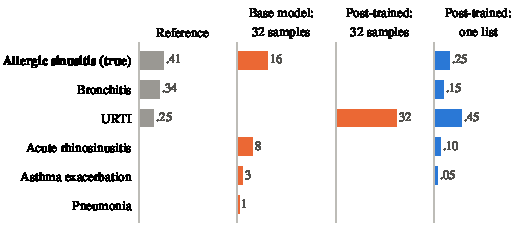
\includegraphics[width=\columnwidth]{fig_example_case.pdf}
\caption{One DDXPlus patient read both ways (zero-shot, temperature 0.7): a 32-year-old man with an itchy nose and throat, a runny nose, a cough and a family history of allergies and asthma (true diagnosis: allergic sinusitis). Qwen3-8B-Base answers allergic sinusitis in 16 of 32 samples (4 invalid). Post-trained Qwen3-8B answers upper respiratory tract infection (URTI, which the reference weights 0.25) in all 32, so pass@32 misses; yet its first stated list names all three reference conditions, allergic sinusitis included.}
\label{fig:example}
\end{figure}

The two readouts agree only for a model that samples from the distribution it states. Instruction-tuned models do not: post-training reduces output diversity~\citep{kirk2024rlhfdiversity}, and such models describe distributions they fail to sample from~\citep{meister2025distributional,jang2026cannotsample}; one aligned answer can list what base-model samples spread across calls~\citep{lake2025overton}, and asking for several answers recovers diversity~\citep{zhang2025verbalized}. This matters clinically. A decision-support system that samples a model several times and defers to a clinician when the answers disagree reads the samples; a clinician reading one answer reads the list (Figure~\ref{fig:example}). We measure both readouts against a clinical reference differential and against case reports' own differentials, and test what the gap does to voting and error signals. Our claim is about measurement, not about whether post-training harms the differential.

\begin{figure*}[t]
\centering
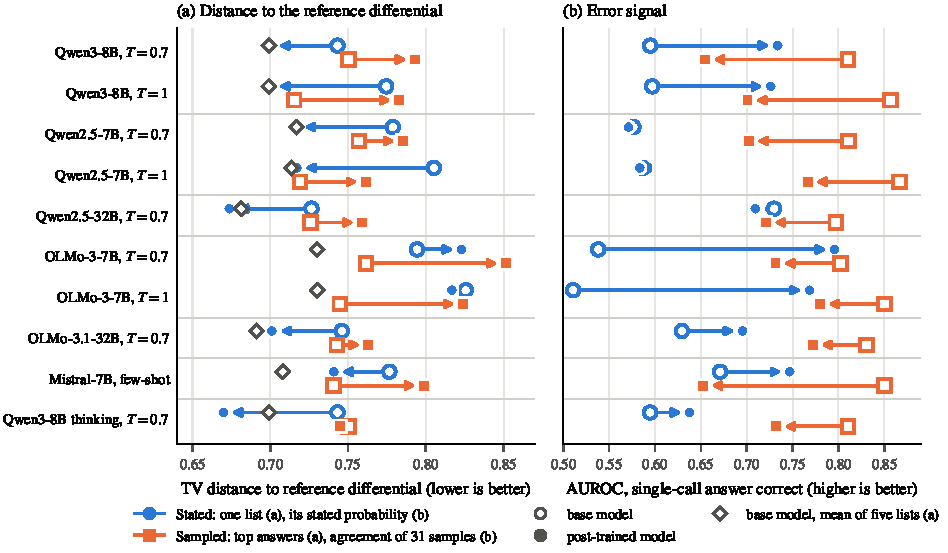
\includegraphics[width=0.82\textwidth]{fig_stated_sampled.pdf}
\caption{Base (hollow) $\rightarrow$ post-trained (filled) on DDXPlus, the first five pairs of Table~\ref{tab:main} at temperature 0.7. (a) Distance to the reference differential (TV, lower is better) of one stated list (blue) and of the 32 sampled answers (orange); grey diamonds: TV of the average of five base-model lists. (b) How well the stated probability (blue) and the agreement of 31 further samples with the first answer (orange) flag whether that answer is correct (AUROC, higher is better).}
\label{fig:main}
\end{figure*}

\section{Setup}
\textbf{Data.} DDXPlus~\citep{fansi2022ddxplus}: 980 synthetic test patients (20 for each of 49 conditions), each with a true diagnosis and a reference differential computed by a rule-based engine; the prompt lists the 49 conditions and asks for the five most likely, with probabilities. A condition is \emph{warranted} if the reference gives it probability at least 0.1. MedCaseReasoning~\citep{wu2025medcasereasoning}: 897 presentations written from open-access case reports, each with the report's final diagnosis; answers are open-ended.

\textbf{Models.} A \emph{base} model is the pretrained network; its \emph{post-trained} version adds instruction tuning and, for most models, preference or reinforcement learning on the same weights. The five main pairs are Qwen3-8B, Qwen2.5-7B, Qwen2.5-32B, OLMo~3 7B and OLMo~3.1 32B~\citep{olmo2025olmo3} (base against final Instruct model). Mistral-7B-v0.3 is secondary, because its base model needs worked examples; Qwen2.5-72B and the medical MedGemma-4B were added later, on DDXPlus only. We draw 32 samples per case at temperature 0.7 (also 1.0 for Qwen3-8B, Qwen2.5-7B and OLMo~3 7B), with Qwen3's reasoning mode off. Base models often ignore a zero-shot instruction, so every DDXPlus pair is also run with three worked examples in the prompt.

\textbf{Readouts.} Each sample is one call returning a ranked list of up to five conditions with probabilities; its first item is the sample's \emph{answer}. The \emph{sampled} readout uses the 32 answers: pass@$k$ (pass@1 is the accuracy of one answer), the number of distinct answers, and their distance to the reference. The \emph{stated} readout~\citep{tian2023justask} scores one list at a time: whether it contains the true diagnosis (recall@5), its distance to the reference, and the share of warranted must-not-miss conditions it names (NSTEMI/STEMI, unstable angina, pulmonary embolism, pneumonia, pulmonary neoplasm, Boerhaave syndrome and spontaneous pneumothorax, from diagnostic-harm data~\citep{newmantoker2024burden} and the chest-pain guideline~\citep{gulati2021chestpain}). Distance is total variation (TV): 0 for identical distributions, 1 for disjoint ones. The \emph{first answer} and \emph{first list} come from a model's first valid sample. An \emph{error signal} flags a wrong first answer: the agreement of the other 31 answers with it, or the probability the model states for it. Invalid answers count as wrong. On the case reports, Mistral-Small-24B-Instruct extracts the alternatives the authors considered and judges whether a name matches one of them or the final diagnosis; Phi-4 gives a strict second grading. Mistral models are therefore not evaluated on these cases.

\textbf{Statistics.} DDXPlus intervals resample the 49 conditions with all their cases. Fourteen metrics in eight settings (the five main pairs at temperature 0.7, three of them also at 1.0), fixed in advance, form the headline tests and are Holm-corrected together; everything else is secondary. Daggers in Table~\ref{tab:main} mark 95\% intervals that include zero; the two 32B pairs' zero-shot pass@32 losses and OLMo~3 7B's case-report loss also do not survive Holm correction. A difference is \emph{equivalent} when its 90\% interval lies within $\pm$5 points.

\section{Results}
\begin{table*}[t]
\centering\small
\setlength{\tabcolsep}{3pt}
\resizebox{\textwidth}{!}{%
\begin{tabular}{lcccccccc}
\toprule
 & \multicolumn{6}{c}{DDXPlus (980 patients, temperature 0.7)} & \multicolumn{2}{c}{Case reports (897)} \\
 & \multicolumn{3}{c}{Sampled top answers} & \multicolumn{3}{c}{Stated (one list)} & \multicolumn{2}{c}{Authors' alternatives covered} \\
 & & & pass@32 change, best & & & & & \\
Pair & pass@1 & pass@32 & prompt: raw / chance-corr. & Recall@5 & TV$\downarrow$ & Must-not-miss & 32 samples & one list \\
\midrule
Qwen3-8B & 0.388 $\rightarrow$ 0.559 & 0.732 $\rightarrow$ 0.607 & $-17.0$ / $-7.7$$^{\dagger}$ & 0.666 $\rightarrow$ 0.802 & 0.743 $\rightarrow$ 0.700 & 0.494 $\rightarrow$ 0.584 & 0.330 $\rightarrow$ 0.190 & 0.300 $\rightarrow$ 0.296$^{\ddagger}$ \\
Qwen2.5-7B & 0.352 $\rightarrow$ 0.478 & 0.695 $\rightarrow$ 0.598 & $-16.3$ / $-10.6$ & 0.573 $\rightarrow$ 0.735 & 0.779 $\rightarrow$ 0.717 & 0.315 $\rightarrow$ 0.536 & 0.376 $\rightarrow$ 0.288 & 0.286 $\rightarrow$ 0.281$^{\ddagger}$ \\
Qwen2.5-32B & 0.500 $\rightarrow$ 0.604 & 0.795 $\rightarrow$ 0.746$^{\dagger}$ & $-15.0$ / $-11.8$ & 0.721 $\rightarrow$ 0.840 & 0.726 $\rightarrow$ 0.674 & 0.432 $\rightarrow$ 0.595 & 0.331 $\rightarrow$ 0.247 & 0.319 $\rightarrow$ 0.318$^{\ddagger}$ \\
OLMo~3 7B & 0.178 $\rightarrow$ 0.265 & 0.705 $\rightarrow$ 0.422 & $-29.9$ / $-17.6$ & 0.470 $\rightarrow$ 0.485$^{\dagger}$ & 0.794 $\rightarrow$ 0.823 & 0.268 $\rightarrow$ 0.413 & 0.351 $\rightarrow$ 0.322 & 0.248 $\rightarrow$ 0.236$^{\ddagger}$ \\
OLMo~3.1 32B & 0.326 $\rightarrow$ 0.560 & 0.796 $\rightarrow$ 0.756 & $-13.2$ / $-7.6$ & 0.652 $\rightarrow$ 0.779 & 0.746 $\rightarrow$ 0.701 & 0.462 $\rightarrow$ 0.459$^{\dagger}$ & 0.359 $\rightarrow$ 0.266 & 0.293 $\rightarrow$ 0.294$^{\ddagger}$ \\
\midrule
Qwen2.5-72B$^{*}$ & 0.530 $\rightarrow$ 0.651 & 0.755 $\rightarrow$ 0.731$^{\dagger}$ & $-12.3$ / $-8.8$ & 0.706 $\rightarrow$ 0.859 & 0.740 $\rightarrow$ 0.681 & 0.468 $\rightarrow$ 0.585 & \multicolumn{2}{c}{\emph{DDXPlus only}} \\
\bottomrule
\end{tabular}}
\caption{Base $\rightarrow$ post-trained models (zero-shot except the best-prompt column; 32 samples per case). Higher is better except for TV. pass@1: accuracy of one sampled answer (invalid answers count as wrong, which mostly penalizes base models). \emph{pass@32 change, best prompt}: post-trained minus base, in percentage points, with each model at the prompt where its own pass@32 is highest (chosen on the test cases; for base models, worked examples), raw and minus a chance baseline (pass@32 scored against another patient's diagnosis). TV: distance of one stated list to the reference differential (0 to 1). Must-not-miss: share of the warranted must-not-miss conditions (reference probability at least 0.1) that one list names, over the seven conditions named in the text. \emph{Authors' alternatives covered}: share of the alternatives the reports' authors considered that any of 32 sampled answers, or one list, names. $^{\dagger}$: the 95\% interval of the change includes zero (condition-clustered bootstrap for DDXPlus, case bootstrap for the case reports); $^{\ddagger}$: equivalent to the base model within 5 points. $^{*}$: added after the tests were fixed.}
\label{tab:main}
\end{table*}

\textbf{Post-training collapses the samples.} Post-trained models give 1.3--2.4 distinct answers per 32 samples, against 3.0--4.9 for their base models, and their samples move away from the reference (Figure~\ref{fig:main}a). They are more accurate on one answer, but the lead shrinks as $k$ grows and reverses before $k{=}16$ in all five main pairs. Compared at each model's best prompt (worked examples for every base model), post-training costs 12--30 points of pass@32 (Table~\ref{tab:main}); subtracting what samples reach by chance leaves 8--18 points in the main pairs (not significant for Qwen3-8B). The collapse is not an artifact of the list prompt: asked for one diagnosis per call, post-trained Qwen3-8B and Qwen2.5-7B give 1.2 and 1.4 distinct answers. Nor is it just a lower temperature: at equal first-answer accuracy, OLMo~3 7B and both 32B post-trained models reach less pass@32 than their base models. And much of the first-answer gain is prompt format: with the same worked examples it shrinks to 2--5 points in four of six pairs.

\textbf{A single stated list keeps its coverage.} A post-trained list still names about five conditions, and zero-shot, for every Qwen model and OLMo~3.1 32B, it contains the true diagnosis 12--16 points more often than the base model's list (Table~\ref{tab:main}). The gains are modest and do not hold for OLMo~3 7B, and five averaged base-model lists get about as close to the reference. What narrows is the variation between calls, and the samples lose what the lists hold: for 7--20\% of patients a post-trained model's 32 answers never include the true diagnosis although its first list does, against about 3\% for base models (Figure~\ref{fig:example}). So in all eight pairs (before correcting for chance), a post-trained model's first list names the true diagnosis more often than its own 32 answers, while a base model's 32 answers beat its list. This reversal is the collapse seen from the list's side, not a better ranking: at equal size, a post-trained list and its samples are within 5.2 points. Post-trained lists also name more of the warranted must-not-miss conditions in seven of eight settings, but still miss about half, and some models lose specific ones.

\textbf{Voting and agreement lose value.} Majority voting over 32 samples raises base models' accuracy by 3.4--8.4 points but post-trained models' by at most 1.9. Agreement flags wrong answers less well after post-training in every pair, significantly for the Qwen models (Figure~\ref{fig:main}b), and it is blind to errors the model repeats: in the eight pairs, every other sample repeats 19--61\% of post-trained models' wrong first answers, against 1--9\% for base models. The stated probability is no fix, flagging only 5--29\% of these silent errors. Which signal works better depends on the model.

\textbf{Real case reports.} The pattern replicates on published cases for the Qwen models and OLMo~3.1 32B: after post-training, 32 samples cover 8--14 points fewer of the alternatives the authors considered, while one list covers as many as before (equivalent within 5 points; Table~\ref{tab:main}). With a closed list of ten candidates graded by name, without a judge model, all four case-report pairs show the gap more sharply. One caveat: for the final diagnosis itself, 32 post-trained samples still beat one list in four of five pairs, so the list is the better source of alternatives, not of the single best answer.

\section{Discussion}
Post-training does not erase a model's differential; it moves it from the samples into the stated list. \textbf{Practical recommendations:}
\begin{itemize}
\item Report whether a metric reads one answer or many samples, and whether the model reasons first.
\item If a system needs several candidates, read them from one stated list, or the union of a few, rather than from repeated samples.
\item Validate agreement-based error signals before trusting them for an instruction-tuned model: choosing between stated probability and agreement on 100 labeled cases picked the better signal in 82\% of draws.
\end{itemize}

\textbf{Limitations.} DDXPlus is synthetic and closed-set: its metrics measure agreement with a rule-based engine, not clinical correctness, and its vignettes lack exam and test results. The case reports are real but graded by judge models, which agree with each other on 97.5\% of names and were checked only against string matches; published cases may appear in pretraining data. We study open 4--72B models with one set of worked examples and no frontier systems, and no clinician reviewed the outputs.

\textbf{Code and data.} Code, prompts and sampled outputs will be released; all data are public. \textbf{Acknowledgments.} An AI assistant (Claude, Anthropic) was used to write analysis code and to draft and edit text; the authors take responsibility for the content.

\bibliography{../paper/refs}

\end{document}
